%\documentclass[12pt,a4paper]{article}
%\documentclass[12pt]{report}
\documentclass[a4paper,14pt]{report}
\usepackage[utf8]{inputenc}
\usepackage[14pt]{extsizes}
\usepackage{listings}
\usepackage{graphicx}
\graphicspath{{schemes/}}
\DeclareGraphicsExtensions{.pdf,.png,.jpg}
\usepackage[english,russian]{babel}
\usepackage{indentfirst}
\usepackage{pdfpages}
\usepackage{titlesec}
\usepackage{amsmath}
\usepackage{float}
\usepackage{caption}
\captionsetup{labelsep=endash}
\captionsetup[figure]{name={Рисунок}}
\newenvironment{comment}{}{}

% Для листинга кода:
\lstset{ %
basicstyle=\small\sffamily, % размер и начертание шрифта для подсветки кода
numbers=right,               % где поставить нумерацию строк (слева\справа)
numberstyle=\tiny,           % размер шрифта для номеров строк
stepnumber=1,                   % размер шага между двумя номерами строк
numbersep=5pt,                % как далеко отстоят номера строк от подсвечиваемого кода
showspaces=false,            % показывать или нет пробелы специальными отступами
showstringspaces=false,      % показывать или нет пробелы в строках
showtabs=false,             % показывать или нет табуляцию в строках
frame=single,              % рисовать рамку вокруг кода
tabsize=4,                 % размер табуляции по умолчанию равен 2 пробелам
captionpos=t,              % позиция заголовка вверху [t] или внизу [b]
breaklines=true,           % автоматически переносить строки (да\нет)
breakatwhitespace=false, % переносить строки только если есть пробел
escapeinside={\#*}{*)}   % если нужно добавить комментарии в коде
}

% Для измененных титулов глав:
\usepackage{titlesec, blindtext, color} % подключаем нужные пакеты
\definecolor{gray75}{gray}{0.75} % определяем цвет
\newcommand{\hsp}{\hspace{20pt}} % длина линии в 20pt
% titleformat определяет стиль
\titleformat{\chapter}[hang]{\Huge\bfseries}{\thechapter\hsp\textcolor{gray75}{|}\hsp}{0pt}{\Huge\bfseries}

%отступы по краям
\usepackage{geometry}
\geometry{verbose, a4paper,tmargin=2cm, bmargin=2cm, rmargin=1.5cm, lmargin = 3cm}
% межстрочный интервал
\usepackage{setspace}
\onehalfspacing
\usepackage{float}
% plot
\usepackage{pgfplots}
\usepackage{filecontents}
\usepackage{amsmath}
\usepackage{tikz,pgfplots}
\usetikzlibrary{datavisualization}
\usetikzlibrary{datavisualization.formats.functions}

\usepackage{graphicx}
\graphicspath{{src/}}
\DeclareGraphicsExtensions{.pdf,.png,.jpg}

\usepackage{indentfirst}
\setlength{\parindent}{1.4cm}
\usepackage{titlesec}
\titlespacing{\chapter}{0pt}{12pt plus 4pt minus 2pt}{0pt}
\renewcommand{\rmdefault}{ftm}

%\def\chaptername{} % убирает "Глава"
%
\includepdf[pages=1]{titul.pdf}


\begin{document}
\fontsize{14}{16pt}

\includepdf[pages=1]{titul.pdf}

\includepdf[pages=2]{titul.pdf}
\def\contentsname{Содержание}
% Титульник
%
\includepdf[pages=1]{titul.pdf}
% Оглавление
\tableofcontents

\newpage
\chapter*{Введение}
\addcontentsline{toc}{chapter}{Введение}
Практически любой вид человеческой деятельности связан с ситуациями, когда имеется несколько возможностей и человек волен из этих возможностей выбрать любую, наиболее подходящую ему.
Задачи наилучшего выбора изучает теория принятия решений. С ее помощью можно
научиться осуществлять выбор более обоснованно, эффективно используя имеющуюся в наличии информацию о предпочтениях. Эта теория помогает избежать принятия заведомо негодных решений и учесть возможные отрицательные последствия непродуманного выбора.

Наиболее обширной задачей многокритериального выбора является задача векторной оптимизации. Применение решений данной задачи может использоваться для экономических, проектных и даже научных задач, в которых нужно достичь оптимального соотношения параметров.

Существует несколько способов решения задачи векторной оптимизации. Целью данной научной работы является изучение данных методов и их анализ.

Можно выделить следующие задачи, необходимые для достижения цели научной работы:
\begin{itemize}
	\item дать определение задаче многокритериального выбора;
    \item сформулировать задачу векторной оптимизации;
    \item сформулировать критерии оценки методов решения;
    \item изучить методы решения задачи;
    \item проанализировать методы решения данной задачи;
    \item составить вывод по проделанной работе.
\end{itemize}

\newpage
\chapter{Анализ предметной области}
В данном разделе будут сформулированы задачи многокритериального выбора и векторной оптимизации, а также будут представлены методы решения задачи векторной оптимизации.
\section{Задача многокритериального выбора}
 Человек в своей
деятельности постоянно сталкивается с ситуациями, в которых ему приходится осуществлять
выбор из множества предложенных. 

Для возможности выбора должен быть задан набор вариантов, из которого следует
осуществлять выбор. Обозначим его $X$ и будем называть множеством возможных решений. 
Отметим что минимальный размер данного множества равен двум, иначе выбора просто не существует. Ограничений сверху на количество возможных решений нет, оно может быть
как конечным, так и бесконечным. При этом природа самих решений не играет никакой роли.
Собственно, выбор решения состоит в указании среди всех возможных такого решения, которое объявляется выбранным. Следует заметить, что нередко происходит выбор не
одного, а целого набора решений, являющегося определенным подмножеством множества
возможных решений $X$. Простейший тому пример, --- когда требуется выбрать несколько человек, претендующих на замещение определенного числа вакантных должностей.
Обозначим множество выбираемых решений $Sel X$. Оно представляет собой решение задачи выбора и им может оказаться любое подмножество множества возможных решений $X$. Таким образом, решить задачу выбора --- означает найти множество $Sel X$.
\begin{equation}
Sel X \subset X
\label{ref:this}
\end{equation}
 Когда множество выбираемых решений не содержит ни одного элемента, выбора не происходит, так как ни одно решение не оказывается выбранным. Подобная ситуация не представляет практического интереса, поэтому множество $Sel X$ должно содержать, по крайней мере, один элемент. В некоторых задачах оно может оказаться бесконечным \cite{formul}.

Суть задачи многокритериального выбора состоит в сокращение множества $X$ возможных выборов до множества $Sel X$ сделанных выборов.

\section{Множество Парето} 
Множеством Парето называется множество оптимальных по Парето выборов.

Пусть существует $f:X \rightarrow R^n$ --- отображение из $X$ на множество $n$ мерных векторов. Каждая из координат вектора является числовой характеристикой критерия выбора. При этом если числовая характеристика одного из критериев выбора $x \in X$ $>$ числовой характеристики того же критерия выбора $x' \in X$, то $x$ является боле предпочтительным чем $x'$ по данному критерию.
 
Назовём $f(x) \geq f(x')$ если каждая координата вектора $f(x) \geq $ соответствующей координаты вектора  $f(x')$.
 
Выбор $x \in X$ называется оптимальной по Парето, если для любого $x' \in X, x' \neq x$, выполняется неравенство $f(x) \geq f(x')$, либо данные выборы не сравнимы. 
 

В случае одного критерия оптимальным по Парето является выбор с максимумом функции $f$. Пример с двумя критериями можно графически показать следующим образом рисунок \ref{pic:par}. 

\begin{figure}[H]
 \center{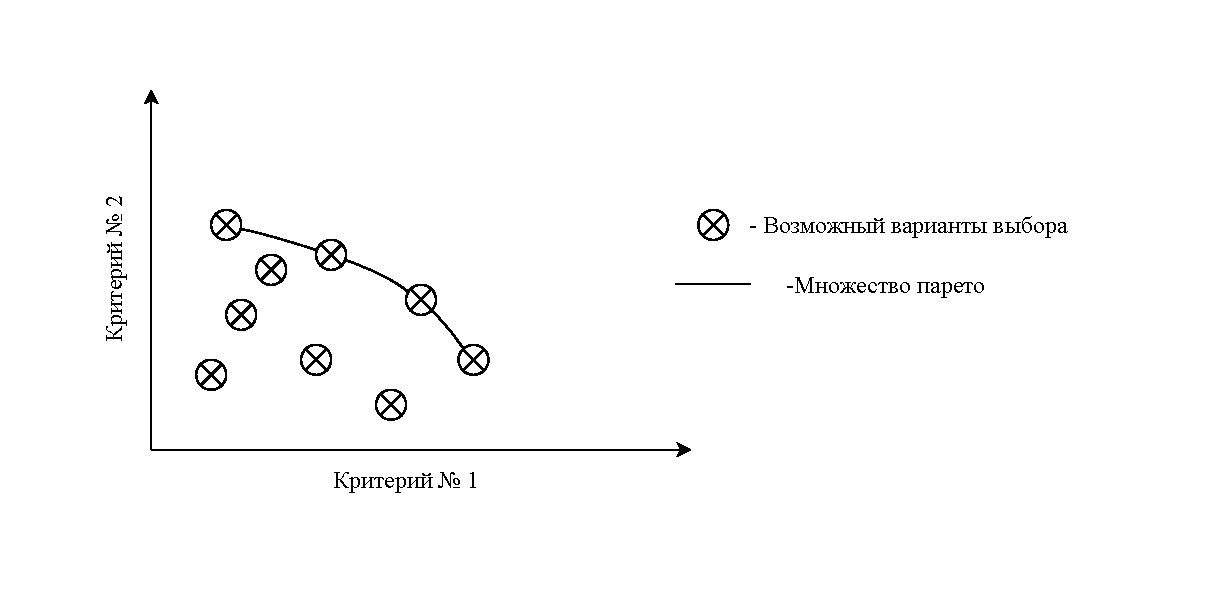
\includegraphics[scale = 0.9]{Pareto.pdf}}
 \caption{Графическое представление множества парето для двух критериев}
 \label{pic:par}
\end{figure}

Множество Парето внутренне устойчиво в том смысле, что в нём не содержится ни одной
такой пары векторов, которые были бы сравнимы по отношению $\geq$.
Это означает, что если при переходе от одного парето-оптимального
вектора к другому происходит увеличение (или уменьшение) какой-то компоненты, то обязательно найдется компонента, по которой
при этом переходе произойдет уменьшение (соответственно --- увеличение) \cite{pareto}.

Отсюда можно сделать вывод что для множества парето все критерии равновесные, и не имеют приоритет.

Множество парето представляет собой множество наиболее оптимальных вариантов выбора. Наиболее удачное решение задачи выбора должно лежать в множестве парето.
Таким образом задача многокритериального выбора сводится к сокращению множества решений до множества парето и выбора решения из данного множества по условиям, заданным лицом принимающим решение (далее --- ЛПР).


\section{Задача векторной оптимизации}
Эффективность функционирования экономической системы оценивается, как правило, несколькими критериями. Математической формой критерия эффективности в оптимизационных экономико-математических задачах является целевая функция.

Векторная оптимизация представляет собой нахождение оптимальных значений по нескольким критериям. Особенность задач векторной оптимизации --- наличие в области допустимых значений области компромиссов, в которой невозможно одновременное улучшение всех критериев.

Пусть существует $n$ параметров $x_i$, таких что $0 \leq x_i \leq c_i$, где $c_i$ --- ограничение сверху.
Обозначим за $x$ вектор $x = (x_1, ... , x_n)$
Критерии представляют собой целевые функции, являющиеся суммой параметров, помноженных на некоторые коэффициенты $f(x) = a_1 * x_1 + ... + a_n * x_n$. Поскольку $f \rightarrow min $ эквивалентно $-f \rightarrow max $, то для простоты в дальнейшем будем предполагать, что все целевые функции необходимо максимизировать. Задача многокритериальной оптимизации в этом случае запишется:

\begin{equation}
\begin{cases}
f_1(x) = \sum\limits_{i=1}^n a_{1,i} * x_i \rightarrow max \\
... \\
f_j(x) = \sum\limits_{i=1}^n a_{j,i} * x_i \rightarrow max \\
... \\
f_m(x) = \sum\limits_{i=1}^n a_{m,i} * x_i \rightarrow max \\
\end{cases}
\label{ref:func}
\end{equation}
при этом 
\begin{equation}
\begin{cases}
0 \leq x_1 \leq c_1 \\
... \\
0 \leq x_i \leq c_i \\
... \\
0 \leq x_n \leq c_n 
\end{cases}
\label{lim}
\end{equation}

Если точки максимума, определенные при решении задач по каждому критерию не совпадают, то решение задачи может быть только компромиссным. В области допустимых значений задачи находится область компромиссов, пример данной области изображён на рисунке \ref{fig:comp}. При перемещении из одной точки области компромиссов в другую, невозможно одновременное улучшение всех критериев. Данная область для задач векторной оптимизации и является множеством Парето, а значит и решение должно лежать в ней \cite{vectorn}.

\begin{figure}[H]
 \center{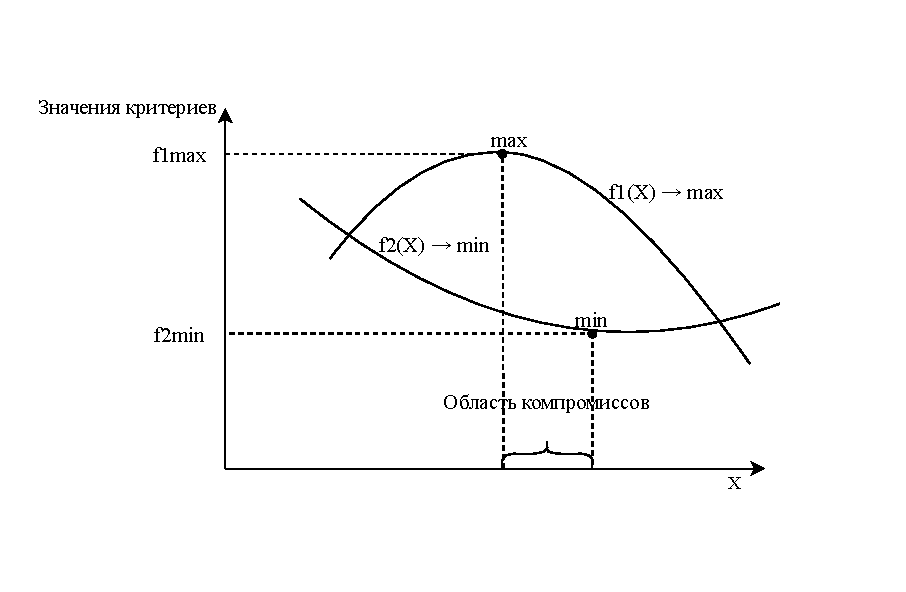
\includegraphics[scale = 1]{Comp.pdf}}
 \caption{Область компромиссов}
 \label{fig:comp}
\end{figure}

\section{Нормализация критериев}
Для решения векторной задачи нередко возникает необходимость к сведению параметров к одинаковым величинам.
Зачастую целевые функции $f(x)$ имеют различную размерность и их необходимо свести к безразмерному виду с помощью какого-нибудь преобразования. Это преобразование должно удовлетворять по крайней мере следующим критериям:
\begin{itemize}
\item иметь общее начало отсчета и один порядок изменения значений на всем множестве допустимых решений;

\item быть монотонным преобразованием, так как множество Парето изменятся не должно;

\item учитывать необходимость минимизации отклонения от оптимальных значений по каждой целевой функции.
\end{itemize}

Обыкновенно для получения нормализованных критериев в качестве таких преобразований используют следующие:

\begin{equation}
f^{n}_i(x) = (f_i(x) - f^{min}_i)/(f^{max}_i - f^{min}_i) \in [0, 1]
\label{ref:lim}
\end{equation}

где , как правило, полагают $f^{min}_i$, $f^{max}_i$ ---  наибольшее и наименьшее значения $i$-го критерия соответственно. 

Нормализация критериев является вспомогательным методом для решения задачи векторной оптимизации.  

\chapter{Классификация существующих методов решений}
Методы решения задач многокритериальной оптимизации можно подразделить на три группы:
\begin{itemize}
\item методы, основанные на свертывании критериев;

\item методы, использующие ограничения на критерии;

\item методы, основанные на отыскании компромиссного решения.
\end{itemize}
Далее будут рассмотрены методы решения задачи векторной оптимизации и критерии их анализа.

\section{Критерии анализа методов}
Недостаток принципа Парето в том, что он предлагает в качестве решения --- множество решений, что не всегда приемлемо. Решение задачи векторной оптимизации для практического применения должно быть одно и при этом принадлежать множеству Парето. Для того, чтобы выбрать из множества Парето единственное решение нужны какие-то дополнительные сведения, предположения, договоренность о том, что же считать наилучшим решением, данные сведения должны задаваться ЛПР. Поэтому для каждого метода необходимо определить какие данные задаются ЛПР.

Необходимо определить, как метод решает проблему учета приоритета критериев которая встает, если критерии имеют различную значимость. 

Для применения методов решения на практике необходимо определить насколько просто реализовать алгоритм этот метод, также для данного алгоритма необходимо определить трудоёмкость в зависимости от числа параметров.

\section{Метод лексикографического решения}
Лексикографическая оптимизация основана на введении отношения порядка критериев по относительной важности. Критерии перенумеровываются таким образом, что функция

$f_1(x)$ считается самым важным показателем, а последняя по номеру функция $f_n(х)$ — наименее важной. Далее рассматривается задача последовательной оптимизации $f_1(x), ..., f_n(х)$. Сначала решается задача $f_1(x) \rightarrow max$ из решения этой задачи получается набор $X^*$ векторов $x$ решения данной задачи. Если набор полученных оптимальных стратегий содержит более одной точки, то решаются задачи $f_2(x) \rightarrow max, ... , f_n(x) \rightarrow max$, до тех пор пока не будут рассмотрены все критерии или найдено единственное решение задачи.

В данном методе приоритет критериев задаётся их порядком, задаваемым ЛПР. Алгоритм метода заключается в последовательном проходе по критериям и вычислении ещё не известных нам параметров. Трудоёмкость данного метода $O(n)$. 



\section{Метод ограничений. Компромиссное решение}


Для метода ограничений следует считать наилучшим такое решение, при котором величина отклонений от оптимальных значений по каждой целевой функции $\Delta{f(x)} = f_i(x) - f_i^{max}$ достигает своего минимального значения. Но наименьшие значения величин, как правило, не достигаются одновременно ни для какого решения.

Поэтому нужны какие-то дополнительные процедуры для отыскания какого-то единственного представителя из множества Парето.  Специфика решения таких задач состоит в том, что сам выбор такой процедуры, метода нахождения окончательного решения в какой-то степени основан на предположениях ЛПР, т. е. на субъективной информации.

Метод ограничений предназначен для отыскания так называемого компромиссного решения, т. е. такого эффективного решения для которого взвешенные относительные потери (потери в смысле разности возможного наилучшего значения целевой функции и значения этой функции для данного --- компромиссного решения) минимальны и равны между собой. 

Метод ограничений основан на теореме: если $x0$ --- эффективное решение для данного вектора предпочтений, то ему соответствует наименьшее значение, при котором система равенств

 выполняется для всех $i = \overline{1,k}$      

При этом под вектором предпочтений понимается некоторый вектор весовых коэффициентов.  Как правило, на него накладываются ограничения С помощью весовых коэффициентов задаются определенные ЛПР предпочтения (значимость) целевых функций (критериев) друг перед другом, выраженные в количественной шкале.

В данном методе приоритет критериев не учитывается, ЛПР задаёт сами процедуры для вычисления компромисса, в этом и заключается основная сложность реализации данного метода. Так как при каждом следующем решение критерия нам нужно учитывать предыдущие то сложность алгоритма будет $O(n^2)$. 

\section{Метод уступок}
Рассмотрим метод, использующих ограничения на критерии --- метод последовательных уступок. 

Алгоритм метода следующий:

1. Критерии нумеруются в порядке убывания важности.

2. Решается задача

\begin{equation}
f_i(x) \rightarrow max
\label{ref:lim}
\end{equation}
\begin{equation}
\begin{cases}
0 \leq x_1 \leq c_1 \\
... \\
0 \leq x_i \leq c_i \\
... \\
0 \leq x_n \leq c_n 
\end{cases}
\label{ref:lim}
\end{equation}

Определяется значение $f^{max}_i$.

3. Устанавливается уступка $\Delta_i$, по этому критерию.

4. Решается задача

\begin{equation}
f_{i+1}(x) \rightarrow max
\label{ref:lim}
\end{equation}
\begin{equation}
\begin{cases}
f_i \geq f^{max}_i - \Delta_i
\begin{cases}
0 \leq x_1 \leq c_1 \\
... \\
0 \leq x_i \leq c_i \\
... \\
0 \leq x_n \leq c_n 
\end{cases}
\end{cases}
\label{ref:lim}
\end{equation}
Данный алгоритм повторяются для всех критериев.
Величины уступок выбирают в пределах инженерной точности, т.е. 5--10\% от наименьшего значения критерия.

Для данного решения критерии оптимальности расположены в порядке убывающей важности. Сначала основной $f_1(x)$, затем другие, вспомогательные: $f_2(x), f_3(x), …$ . Сначала ищется решение, обращающее в максимум главный критерий оптимальности $f_1(x)$.  Затем назначается, исходя из практических соображений и точности, некоторая «уступка» $\Delta$, которую ЛПР согласно допустить для того, чтобы обратить в максимум второй показатель $f2(x)$. Налагаем на критерий $f1(x)$ ограничение, чтобы он был не меньше, чем $f^{max}_1 - \Delta * f^{max}_1$, где $f^{max}_1$ --- максимально возможное значение $f_1(x)$, и при этом ограничении ищем решение, обращающее в максимум $f_2(x)$. Далее снова назначается «уступка» в показателе $f_2(x)$, ценой которой можно максимизировать $f_3(x)$, и т. д.

Такой способ построения предпочтительного решения хорош тем, что здесь сразу видно, ценой какой «уступки» в одном показателе приобретается выигрыш в другом. Надо сказать, что свобода выбора решения, приобретаемая ценой даже незначительных «уступок», может оказаться существенной, так как в районе максимума обычно эффективность решения меняется очень слабо.

В данном методе приоритет критериев задаётся их порядком. ЛПР задаёт порядок критериев и уступки по каждому из критериев. Трудоёмкость данного метода $O(n^2)$, так как нам необходимо учитывать предыдущие уступки для каждого следующего критерия. 

\section{Метод свертки}
В методах, основанных на свертывании критериев, из локальных критериев формируется один. Наиболее распространенным является метод линейной комбинации частных критериев. Данный метод применим, так как чтобы максимизировать сумму нам нужно максимизировать каждое из слагаемых. Линейная скаляризованная функция представляет собой сумму частных критериев. Задача математического программирования становится однокритериальной и имеет вид


\begin{equation}
f(x) = \sum\limits_{i=1}^m f_i \rightarrow max \\
\label{ref:func}
\end{equation}


Также при использовании данного метода можно задать важность критериев установив для них веса $k_1 , ... , k_m$. В таком случае линейная скаляризованная функция представляет собой сумму частных критериев, помноженных на коэффициенты.

\begin{equation}
f(x) = \sum\limits_{i=1}^m f_i * k_i \rightarrow max \\
\label{ref:func}
\end{equation}

Критерии в свертке могут быть предварительно нормированы. Решение, полученное в результате оптимизации получившегося критерия эффективно.

Далее мы можем узнать, как изменяется функция от конкретного параметра и выбрать для этого параметра максимальное значение или минимальное.

К недостаткам метода можно отнести то, что малым приращениям коэффициентов соответствуют большие приращения функции, т. е. решение задачи неустойчиво, а также необходимость определения весовых коэффициентов.
Метод свертки, идея которого состоит в построении на основе заданных k целевых функций единой целевой функции, является одним из первых в хронологии появления методов решения многокритериальных задач, пожалуй, самым простым и самым распространенным.  

Тем не менее, этому методу присущи определенные свойства, в силу которых метод не всегда позволяет получить адекватное представление об эффективных решениях задачи.

Применение метода свертки с использованием линейной функцией свертки существенно сужает множество получаемых эффективных решений по сравнению со всем множеством Парето. Изменения коэффициентов предпочтения ситуацию не изменяют \cite{vecopt}.

Так же, как и метод ограничений, метод свертки предполагает использование субъективной информации ЛПР в виде коэффициентов предпочтения, однако тут оно задаётся с помощью весовых коэффициентов. Надо отметить, что при решении реальных задач определение этих коэффициентов представляет собой не простую задачу.
Трудоёмкость данного метода $O(n)$, так как нам необходимо сложить все критерии в один и решить полученный критерий.  

\section{Вывод}
Решение получаемое с помощью каждого из методов лежат в множестве парето, однако решения, получаемые с помощью различных методов могут оказаться отличными друг от друга. Это происходит в следствии использования разных способов установки приоритета критериев и разных стратегиях, используемых методами при нахождении наилучшего решения. Таким образом для решения конкретной задачи необходимо выбрать метод наиболее подходящий для её решения. 
Наиболее простым для реализации и наименее трудоёмким являются методы свёртки и лексикографического решения. В методе ограничений ЛПР самому необходимо определить метод установки ограничений.


\chapter{Заключение}
Так или иначе, при любом способе формализации, задача количественного обоснования решения по нескольким показателям остается не до конца определенной, и окончательный выбор решения определяется волевым актом ЛПР. Дело исследователя --- предоставить в распоряжение ЛПР необходимые расчеты, позволяющие лицу, принимающему решение всесторонне оценить преимущества и недостатки каждого варианта решения и, опираясь на них, сделать окончательный выбор.

В результате выполнения работы было дано определение задаче многокритериального выбора, сформулирована задача векторной оптимизации, сформулированы критерии оценки методов решения, изучены и проанализированы методы решения данной задачи и составлен вывод по проделанной работе. Цель научной работы была достигнута.

\renewcommand\bibname{Список литературы}
\addcontentsline{toc}{chapter}{Список литературы}
\makeatletter % список литературы
\def\@biblabel#1{#1. }
\makeatother
\begin{thebibliography}{2}
	\bibitem{formul} Ногин В.Д. Принятие решений в многокритериальной среде: Наука. Гл. ред. физ.-мат. лит. 2005.
    \bibitem{vectorn} Коротченко А.Г. Кумагина Е.А. Сморякова В.М. Введение в многокритериальную оптимизацию: Гл. ред. Нижегородского государственного университета
им. Н.И. Лобачевского 2017.
	\bibitem{} Подиновский В.В. Ногин В.Д. Парето-оптимальные решения многокритериальных задач. М.: Наука. Гл. ред. физ.-мат. лит. 1992.
	\bibitem{vecopt} Машунин Ю.К. Векторная оптимизация. Том 2. Векторная оптимизация в инженерии: Русайнс 2021.
	\bibitem{pareto} Ногин В.Д. Множество и принцип Парето:194021, Санкт-Петербург, Политехническая ул., д. 24, лит. В, пом. 11-Н № 25, 26. 2020.
	\bibitem{} Диалло А.Б., Дим Д.Т., Бакасов С.Р., Богатиков В.Н. Использование «метода уступок»  // Вестник Евразийской науки, 2018 URL:
https://esj.today/PDF/25ECAVN118.pdf (доступ свободный). Загл. с экрана. Яз. рус., англ.(дата обращения: 27.12.2021)
\end{thebibliography}

\end{document}

